\begin{center}
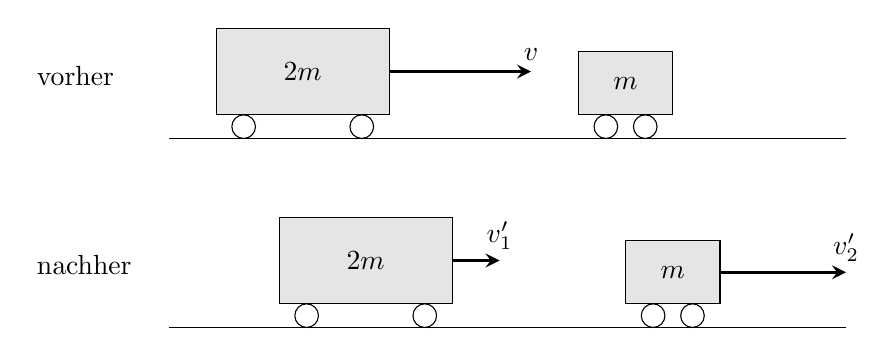
\begin{tikzpicture}[>=stealth]
 \node[anchor=west] at (0,0.8) {vorher};
 \draw (1.8,0) -- (10.4,0);
 \draw[fill=gray!20] (2.4,0.3) rectangle (4.6,1.4);
 \node at (3.5,0.85) {$2m$};
 \draw[fill=white] (2.75,0.15) circle (0.15) (4.25,0.15) circle (0.15);
 \draw[->, very thick] (4.6,0.85) -- (6.4,0.85) node[above] {$v$};
 \draw[fill=gray!20] (7,0.3) rectangle (8.2,1.1);
 \node at (7.6,0.7) {$m$};
 \draw[fill=white] (7.35,0.15) circle (0.15) (7.85,0.15) circle (0.15);
 \node[anchor=west] at (0,-1.6) {nachher};
 \draw (1.8,-2.4) -- (10.4,-2.4);
 \draw[fill=gray!20] (3.2,-2.1) rectangle (5.4,-1);
 \node at (4.3,-1.55) {$2m$};
 \draw[fill=white] (3.55,-2.25) circle (0.15) (5.05,-2.25) circle (0.15);
 \draw[->, very thick] (5.4,-1.55) -- (6,-1.55) node[above] {$v_1'$};
 \draw[fill=gray!20] (7.6,-2.1) rectangle (8.8,-1.3);
 \node at (8.2,-1.7) {$m$};
 \draw[fill=white] (7.95,-2.25) circle (0.15) (8.45,-2.25) circle (0.15);
 \draw[->, very thick] (8.8,-1.7) -- (10.4,-1.7) node[above] {$v_2'$};
\end{tikzpicture}
\end{center}

Mit $v = \vWaO$ und den Geschwindigkeiten $v_1'$ (Masse $2m$) und $v_2'$ (Masse $m$) nach dem Stoss gelten
\begin{align}
 \text{Impuls:}\quad 2m\,v &= 2m\,v_1' + m\,v_2' &&\Rightarrow\quad v_2' = 2\left(v-v_1'\right) \\
 \text{Energie:}\quad \frac{1}{2}\cdot 2m\,v^2 &= \frac{1}{2}\cdot 2m\,{v_1'}^2 + \frac{1}{2}m\,{v_2'}^2 &&\Rightarrow\quad 2v^2 = 2{v_1'}^2 + {v_2'}^2
\end{align}
Einsetzen von $v_2'$ in die Energiegleichung:
\begin{align}
 2v^2 &= 2{v_1'}^2 + 4\left(v-v_1'\right)^2 \\
 0 &= 3{v_1'}^2 - 4v\,v_1' + v^2 = \left(3v_1'-v\right)\left(v_1'-v\right)
\end{align}
Die Lösung $v_1' = v$ beschreibt den Fall ohne Stoss. Die gesuchte Lösung ist
\begin{align}
 v_1' &= \vEnF = \frac{\vWa}{3} = \vEn \approx \result{\vEnP{0}{2}} \\
 v_2' &= 2\left(v-\frac{v}{3}\right) = \vZnF = \frac{4\cdot\vWa}{3} = \vZn \approx \result{\vZnP{0}{2}}
\end{align}
Beide Wagen fahren in der ursprünglichen Richtung weiter, der leichtere schneller. Dasselbe liefern die Formeln für den elastischen Stoss (FoTaBe S.~159).
